\documentclass{article}

\usepackage[utf8]{inputenc}
\usepackage[a4paper, total={6in, 8in}]{geometry}
\usepackage{amsmath,mathtools,amstext,array,cases,biblatex,float,tikz}
\usepackage[T1]{fontenc} 
\usepackage{microtype} 

\newcolumntype{L}{>{$}l<{$}}
\addbibresource{biblio.bib}
\def\labelitemi{--}
\usetikzlibrary{arrows,positioning}


\begin{document}

\title{Chapter 1}

\author{M. Repetto}

\date{\today}

\maketitle

\begin{abstract}
This chapter deals with the problem of multinational entity allocation based on three main factors, namely the costs, the
tax pressure and the functional characterization of a certain entity. The solution suggested is a goal programming model that embeds this limitation imposed by the environment and tries to find an optimal solution that permits the Decision Maker to be competitive \textit{vis-à-vis} multinational competitors.
\end{abstract}

\section{Introduction}
After the Great Recession, multinational companies found themselves in a very different environment; thriving to survive with competition on one side and higher restriction imposed by countries running financial crises. This led multinationals with a great challenge which consequently boost cost engineering, in an attempt to survive in this new scenario. Another result was a new form of tax planning, most of the time barely legal in order to exploit the fiscal advantages of certain countries\cite{_after_tax_hedging_report.pdf_????}. Such problems forced the G20 to launch an inclusive framework on base erosion and profit shifting called "BEPS", bringing together about 100 countries in order to stop such unlawful tax planning. However, even if this action against such problem highlighted in a more specific way what should be considered as aggressive tax planning the border with legitimate cost engineering seems blurrier than ever\cite{feller_three_2017}.
In this paper, I'll try to build a model that given a set of criteria based on the accounting information of a specific multinational, it tries to perform the best allocation of its entities. The model will use both internal and external data and will follow three main objectives, namely minimize the costs, minimize the tax base and at the same time be compliant with its functional characterization, meaning that its profitability is in line with independent actor in the market \cite{_model_2015} and it's not a mere result of aggressive tax planning.

\begin{figure}[htb!]
\centering
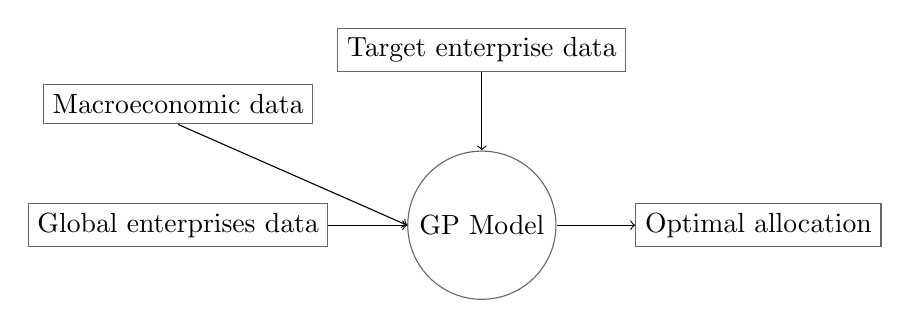
\begin{tikzpicture}[
squarednode/.style={rectangle, draw=black!60, minimum size=5mm},
circlenode/.style={circle, draw=black!60, minimum size=5mm},
]

\node[circlenode]      (maintopic)                              {GP Model};
\node[squarednode]        (t1)       [above=of maintopic] {Target enterprise data};
\node[squarednode]      (t2)       [right=of maintopic] {Optimal allocation};
\node[squarednode]        (t3)       [left=of maintopic] {Global enterprises data};
\node[squarednode]        (t4)       [above=of t3] {Macroeconomic data};

\draw[->] (t1.south) -- (maintopic.north);
\draw[->] (t4.south) -- (maintopic.west);
\draw[->] (t3.east) -- (maintopic.west);
\draw[->] (maintopic.east) -- (t2.west);
\end{tikzpicture}
\caption{Model flowchart}
\end{figure}

The following sections are organized as follows; the first part is an introduction to multi-criteria analysis and more specifically to the Goal Programming approach; the second part is a state of the art review of the fields in where GP was applied so far; the third part will be about the data that led to the model; the fourth will be about the formulation of such model taking into account the possible constraints and then the conclusion and possible limitations of such model.

\section{Multi-criteria decision analysis}
Even if the practice of decision making is old as man, we tend to date the roots of modern MCDA in the early 60's, the main focus at the time was to find the most preferred solution, or generating an approximation to the entire efficient frontier\cite{greco_multiple_2016}.
\\
Multi-criteria analysis may be defined as a problem of multiple-objective programming, that differs from a linear one,
since we have more objective functions to deal with; its formulation is the following:

\[
Min[f_1(x),f_2(x),...,f_k(x)] \quad i=1,...,k \quad where \quad k\geq2
\]

This approach seems to fit better the real world since, in reality, we tend to have a more than one objective most of the time in contrast with one another. 
A solution to a multi-criteria problem would be optimal if it'd respected the Pareto Efficient assumption, namely that no other feasible solution exists that is at least as good with respect to all objectives and strictly better with respect to at least one objective. Mathematically it means that $\left\{x_1,...x_k\right\}$ is a solution if $\not\exists \left\{x'_1,...x'_k\right\}$
such that:
\[
g(f_1(x),f_2(x),...,f_k(x)) \leq g(f_1(x'),f_2(x'),...,f_k(x')) \quad \forall n \quad \in  \left\{1...k\right\}
\]

Now that we grasped the concept of a multi-criteria problem it's worth saying that there are many approaches to solve such problem, one of these is the Goal Programming, which develops from the concept of linear programming.
\\
Goal Programming, hereinafter GP, is a multi-criteria decision analysis approach which allows the decision maker to consider simultaneously several conflicting objectives.

The idea behind such method is very simple, and is based on distance minimization; this means that at each objective function is associated a deviation variable that has to be minimized in batch with the other deviation variables coming from the other objective functions.

Such models may be represented algebraically as follows:


\[
Min \quad a=h(n,p) \quad s.t: \quad 
\begin{cases}
f_q(x)+n_q-p_q=b_q \\
x\in F \\
n_q,p_q\geq 0
\end{cases}
\]

GP is vastly applied in many fields\cite{tamiz_goal_1998} such as management, engineering, and social sciences. Its origins are dated back to the 50's, firstly introduced by Abraham Charnes and William Cooper\cite{charnes_optimal_1955} with an article on the optimal estimation of executive compensation. 

In such approach, we can distinguish three main different categories, namely the lexicographic GP, the weighted GP and the Chebyshev GP.

Lexicographic GP, also named “preemptive” Goal Programming, distinguish itself from the other GP techniques as it has a number of priority levels chosen a priori. The mathematical formulation is the following one:
\[
Lex \quad Min \quad [h_1(n,p),...,h_L(n,p)]
\]

\[
\begin{cases}
f_q(x)+n_q-p_q=b_q & q=1,...Q
\\
x\in F
\\
n_q,p_q\geq0 & q=1,...,Q
\end{cases}
\]

As opposed to LGP, the WGP allows for direct trade-offs between all unwanted deviational variables by using weight that are not putted a priori (as the LGP), as a result WGP is more flexible but as counter-effect it requires more computational power.The mathematichal formulation is the following one:
\[
Min \quad \sum_{q=1}^{Q}(\frac{u_q n_q}{k_q}+\frac{v_q n_q}{k_q})
\]

\[
\begin{cases}
f_q(x)+n_q-p_q=b_q & q=1,...Q
\\
x\in F
\\
n_q,p_q\geq0 & q=1,...,Q
\end{cases}
\]

The last GP variant, presented by Flavell. It differs from the first two variants since it uses the underlying $ L_\infty $ means of measuring distance. Also called Minmax goal programming it seeks to minimize the maximal deviation from any goal. Therefore the primary goal of such approach is the balance. The mathematical formulation is the following one:
\[
Min \quad \lambda
\]

\[
\begin{cases}
f_q(x)+n_q-p_q=b_q & q=1,...Q
\\
\frac{u_q n_q}{k_q}+\frac{v_q n_q}{k_q}\leq\lambda & q=1,...Q
\\
x\in F
\\
n_q,p_q\geq0 & q=1,...,Q
\end{cases}
\]

\section{A state of the art review in accounting}
As highlighted by Aouni\cite{aouni_goal_2017}, generally accountants are facing complex decision-making situations where they aggregate simultaneously several conflicting and incommensurable factors. This means that GP may become a very useful aid tool in hands of accountants to perform such decisions. Many GP models have been created to solve a broad range of accounting topics such as in audit sampling\cite{tayi_integration_1985} or other fields dealing with management accounting such as pricing\cite{tan_multipleobjective_2008}, costing\cite{dowlatshahi_product_2001}, capital budgeting and performance evaluation\cite{hung_integrated_2011}.
This popularity is due to the fact that GP is easy to understand and to apply, plus it facilitates consideration of trade-off in the decision-making process.
Aside from its popularity, the interest of academics in international tax planning never arose,
it’s worth mentioning the work of Merville and Petty\cite{merville_transfer_1978} who tried to model an optimal pricing policy which is indeed useful to set a global tax
strategy since the TP core is base on that.
The two main variants concerning GP in accounting are Lexicographic GP and Weighted GP, with the first one over topping from the second.

\section{Model formulation}

\subsection{Data used to formulate the model}
The data used in this particular GP model comes from different sources and they can be summarized in the following categories:
\begin{itemize}
    \item Macroeconomic data;
    \item Target enterprise data;
    \item Global enterprises data.
\end{itemize}

\subsubsection{Macroeconomic data}
The group of Macroeconomic data includes the Corporate Tax Rate defined as "the percentage on corporate income generated deemed to the State". The Figure 2 below shows how this rate is different from State to State. This means that different allocation of corporate entities may result in an advantage from a competitive perspective. For example, a new allocation from Germany to Estonia may result in a gain in terms of income of +30\% on net income that may be reinvested in the company.  

The second Macroeconomic data is the Gross National Income per capita. This kind of index is a good proxy for the average cost of an employee per year which instead is computed by dividing the national-accounts-based total wage bill by the average number of employees in the total economy, which is then multiplied by the ratio of the average usual weekly hours per full-time employee to the average usually weekly hours for all employees. The latter indicator was not chosen since it computed in very few countries (the OECD countries) and doesn't permit to obtain a full range of choice by the model. Figure 3 reported below shows the geographical distribution of such index from state to state.

\begin{figure}[ht]
\centering
\begin{minipage}{.5\textwidth}
  \centering
  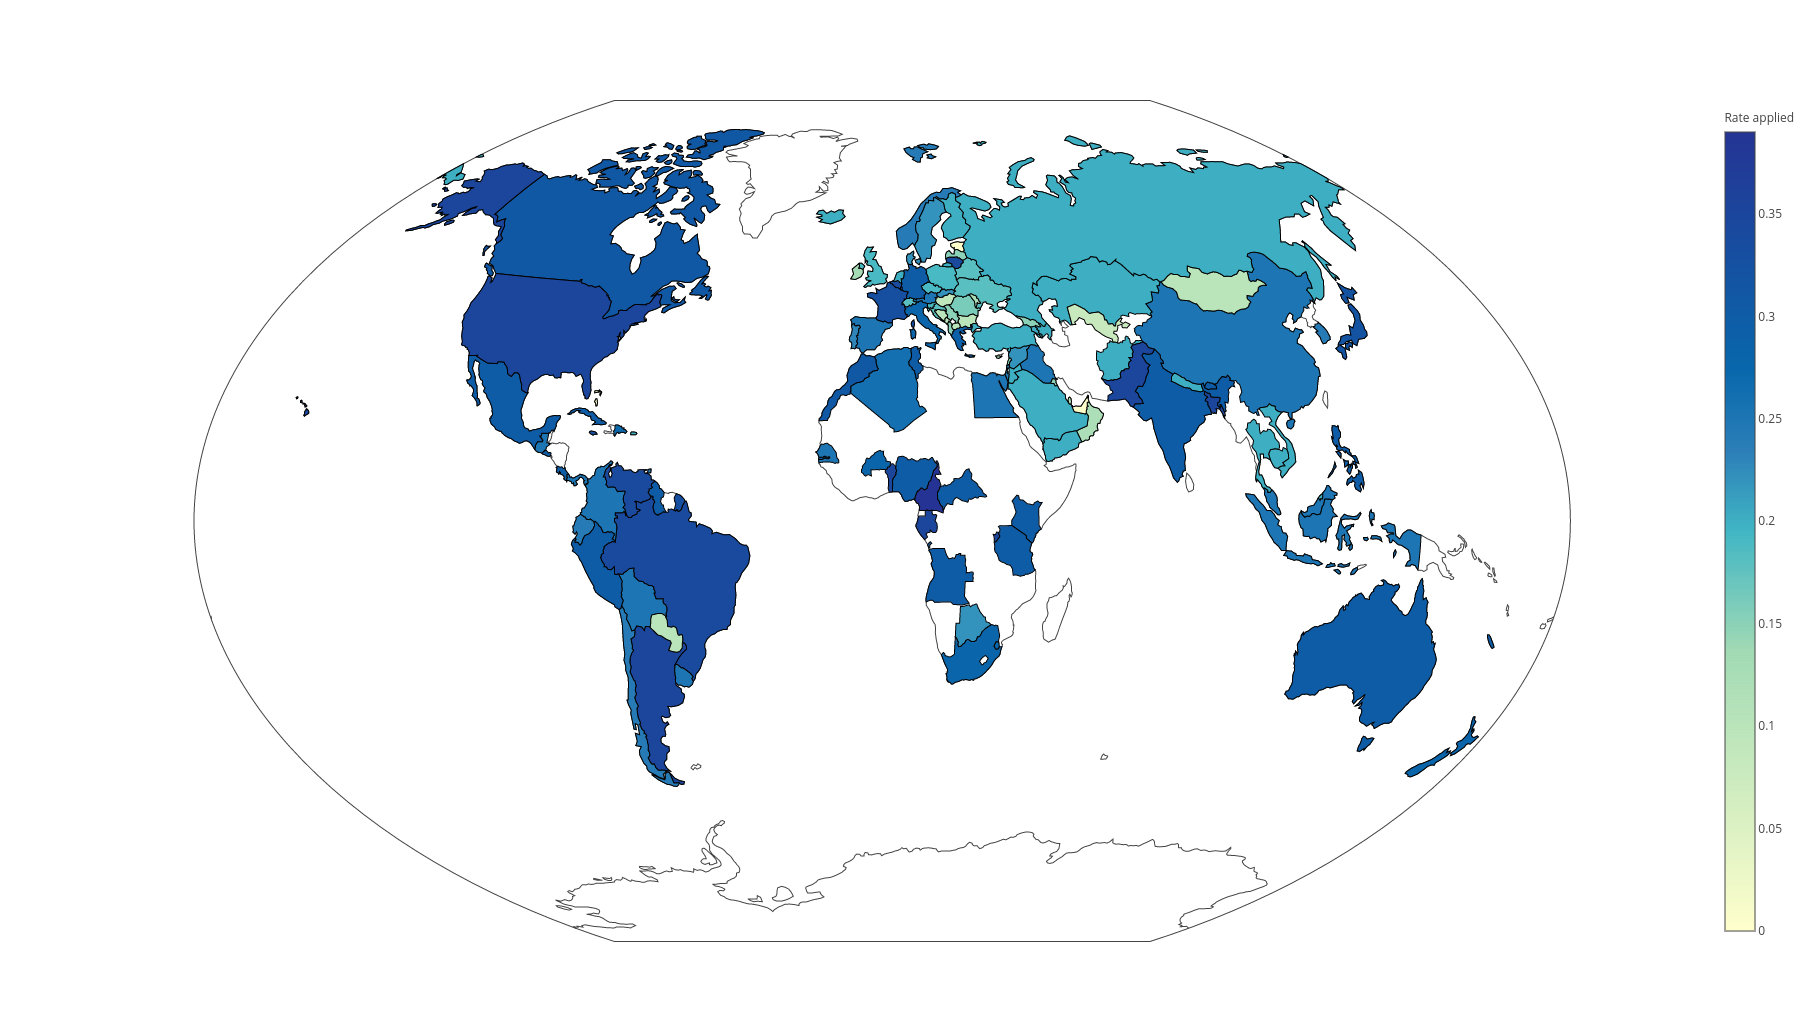
\includegraphics[width=1\linewidth]{Images/CTworld.png}
  \caption{Corporate Tax around the world}
  \label{fig:test1}
\end{minipage}%
\begin{minipage}{.5\textwidth}
  \centering
  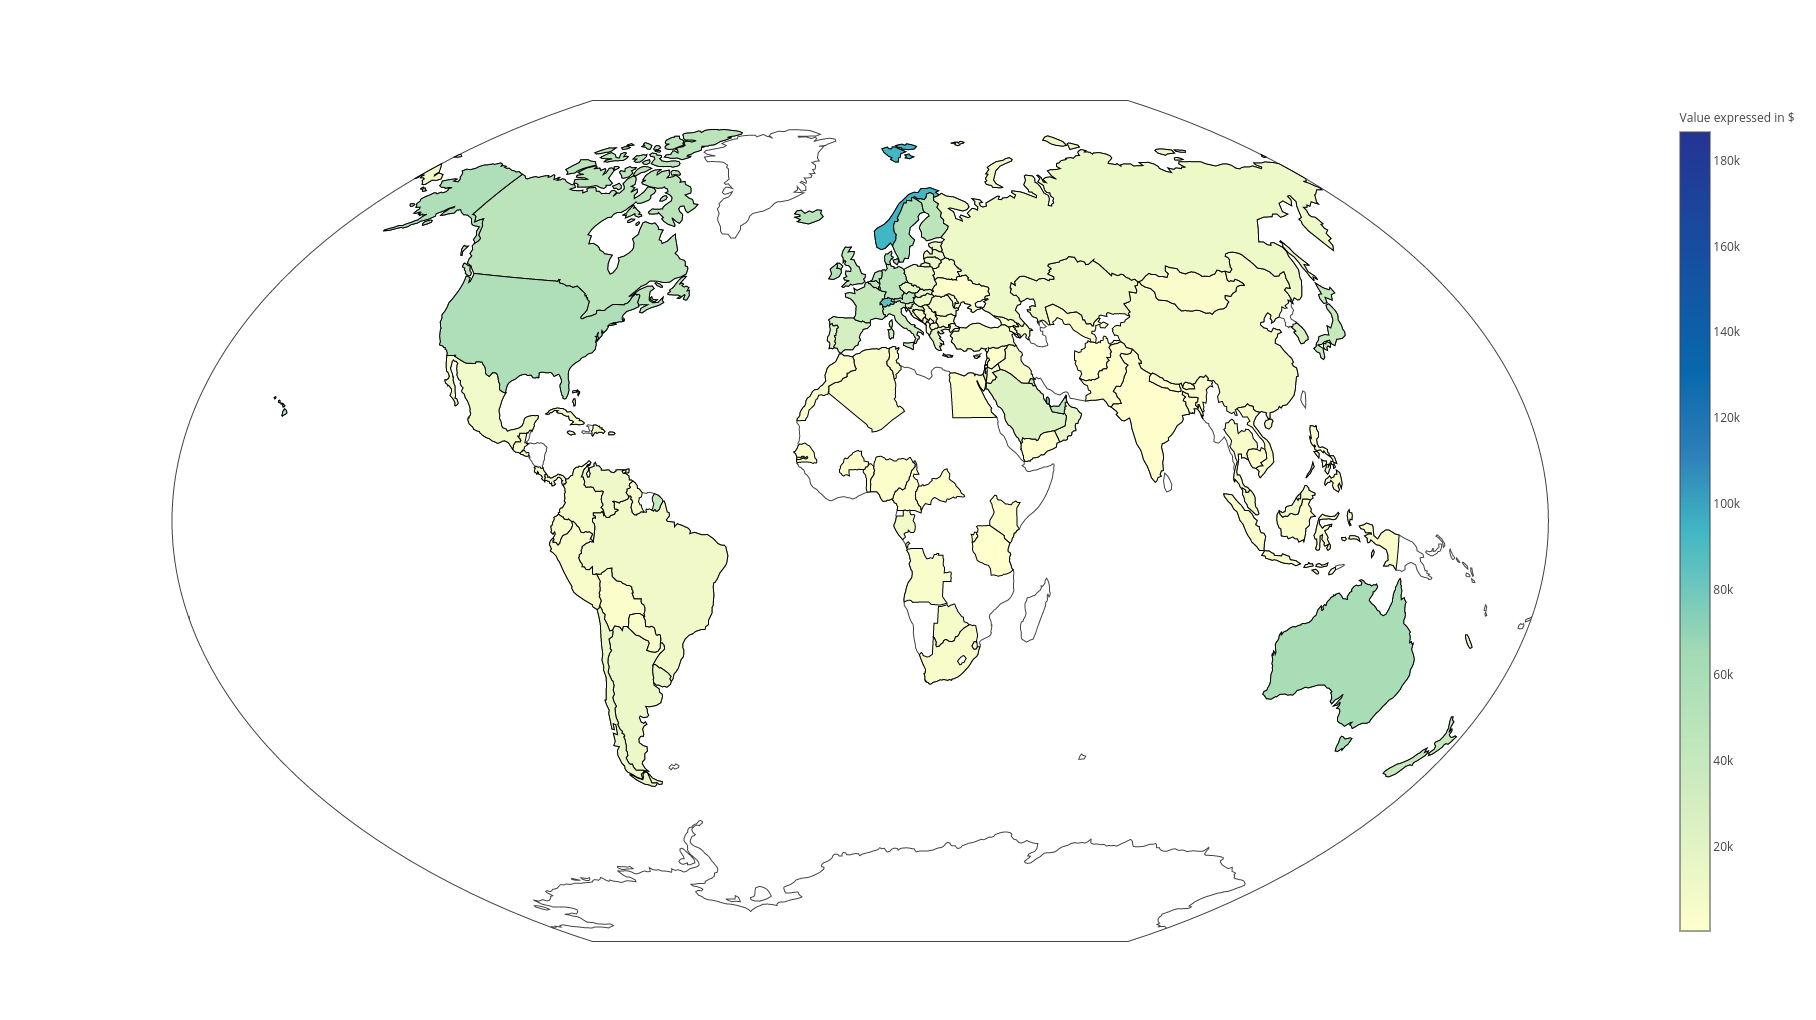
\includegraphics[width=1\linewidth]{Images/GNIworld.png}
  \caption{Gross National Income per capita}
  \label{fig:test2}
\end{minipage}
\end{figure}

\begin{figure}[ht]
\centering
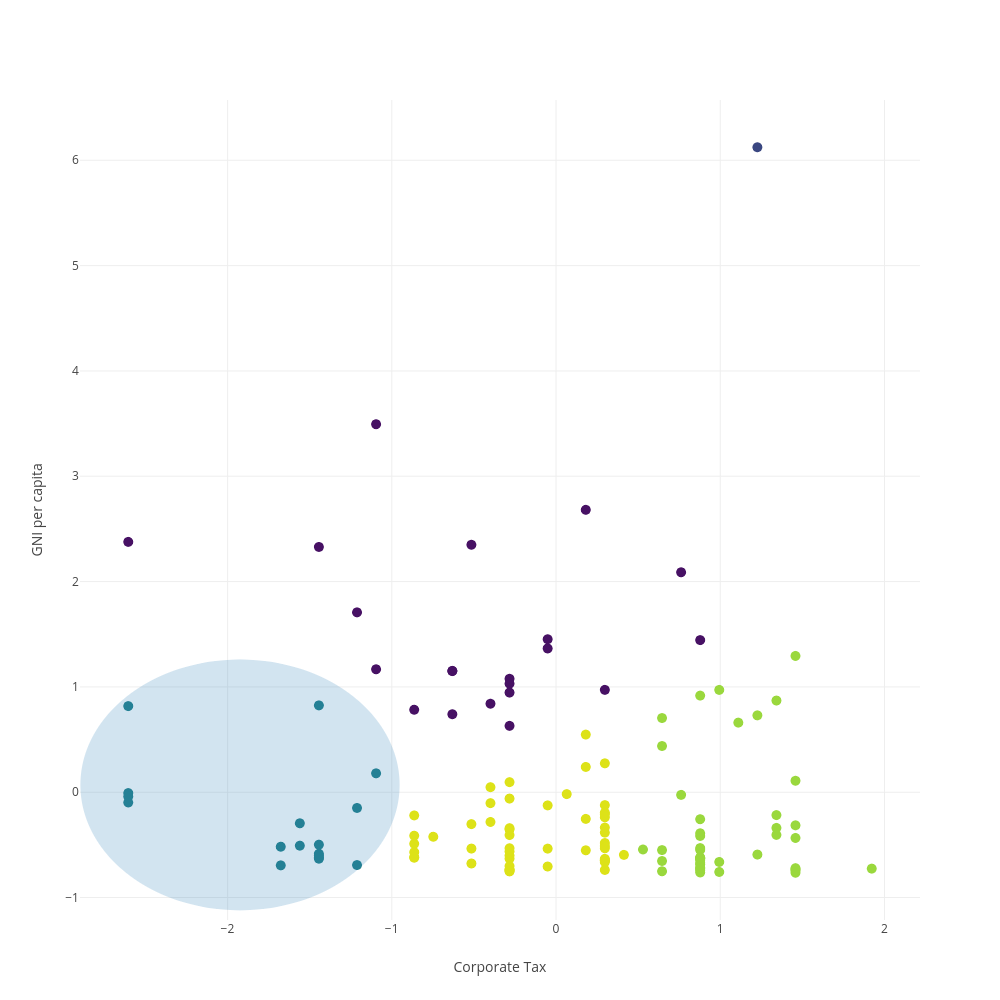
\includegraphics[width=0.8\linewidth]{Images/Cluster-GNI-CT.png}
\caption{K-mean cluster on standardized Corporate Tax and GNI per capita}
\end{figure}

Figure 4 shows a scatter plot of the normalized Corporate Tax (x axis) and GNI per capita (y axis), to such data I applied a K-mean cluster algorithm with K=5, this kind of algorithm randomly assigns each observation to a cluster, and finds the centroid of each cluster then, through iteration reassign data points to the cluster whose centroid is closest and calculate the new centroid of each cluster. The K was chosen with the "elbow method" with $R^2$ meaning that 5 was the number of cluster that return the best trade off in terms of $R^2$ increase and and cluster numerosity. 
The result were five clusters with the one highlighted by the circle indicating countries with both a low average cost of worker and a low taxation. However even if these may seem the best locations to allocate the entities this is not always true, since the formula for taxation is the one proposed at section 4.2 and such entities have to be in the range proposed in section 4.3. 

\subsubsection{Target enterprise data}
This data includes the information we got from our enterprise (the one in which we're going to reallocate the entities). This piece of information are the revenues, the operating expenses. From the operating expenses less wages we can obtain the information inherent the cost of running the assets\cite{williams_financial_2008}, we can then adjust this information with the purchasing parity to obtain the cost of assets from country to country. 

\subsubsection{Global enterprises data}
This category contains all the data inherent the PLI of the specific functional enterprises operating in a certain State.
A piece of this data is summarized by the following representation. Another important data that can be obtained is the cost of debt \cite{berman_financial_2013} even though such measure has to take into account the proportion of two types of funding (namely equity and debt) the data provided by the comparable enterprises serve as a good proxy for such measure if used in conjunction with financial databases as Bloomberg. In our case, to obtain this data a private worldwide database was used called Orbis by Bureau Van Dijk.

\begin{figure}[H]
\centering
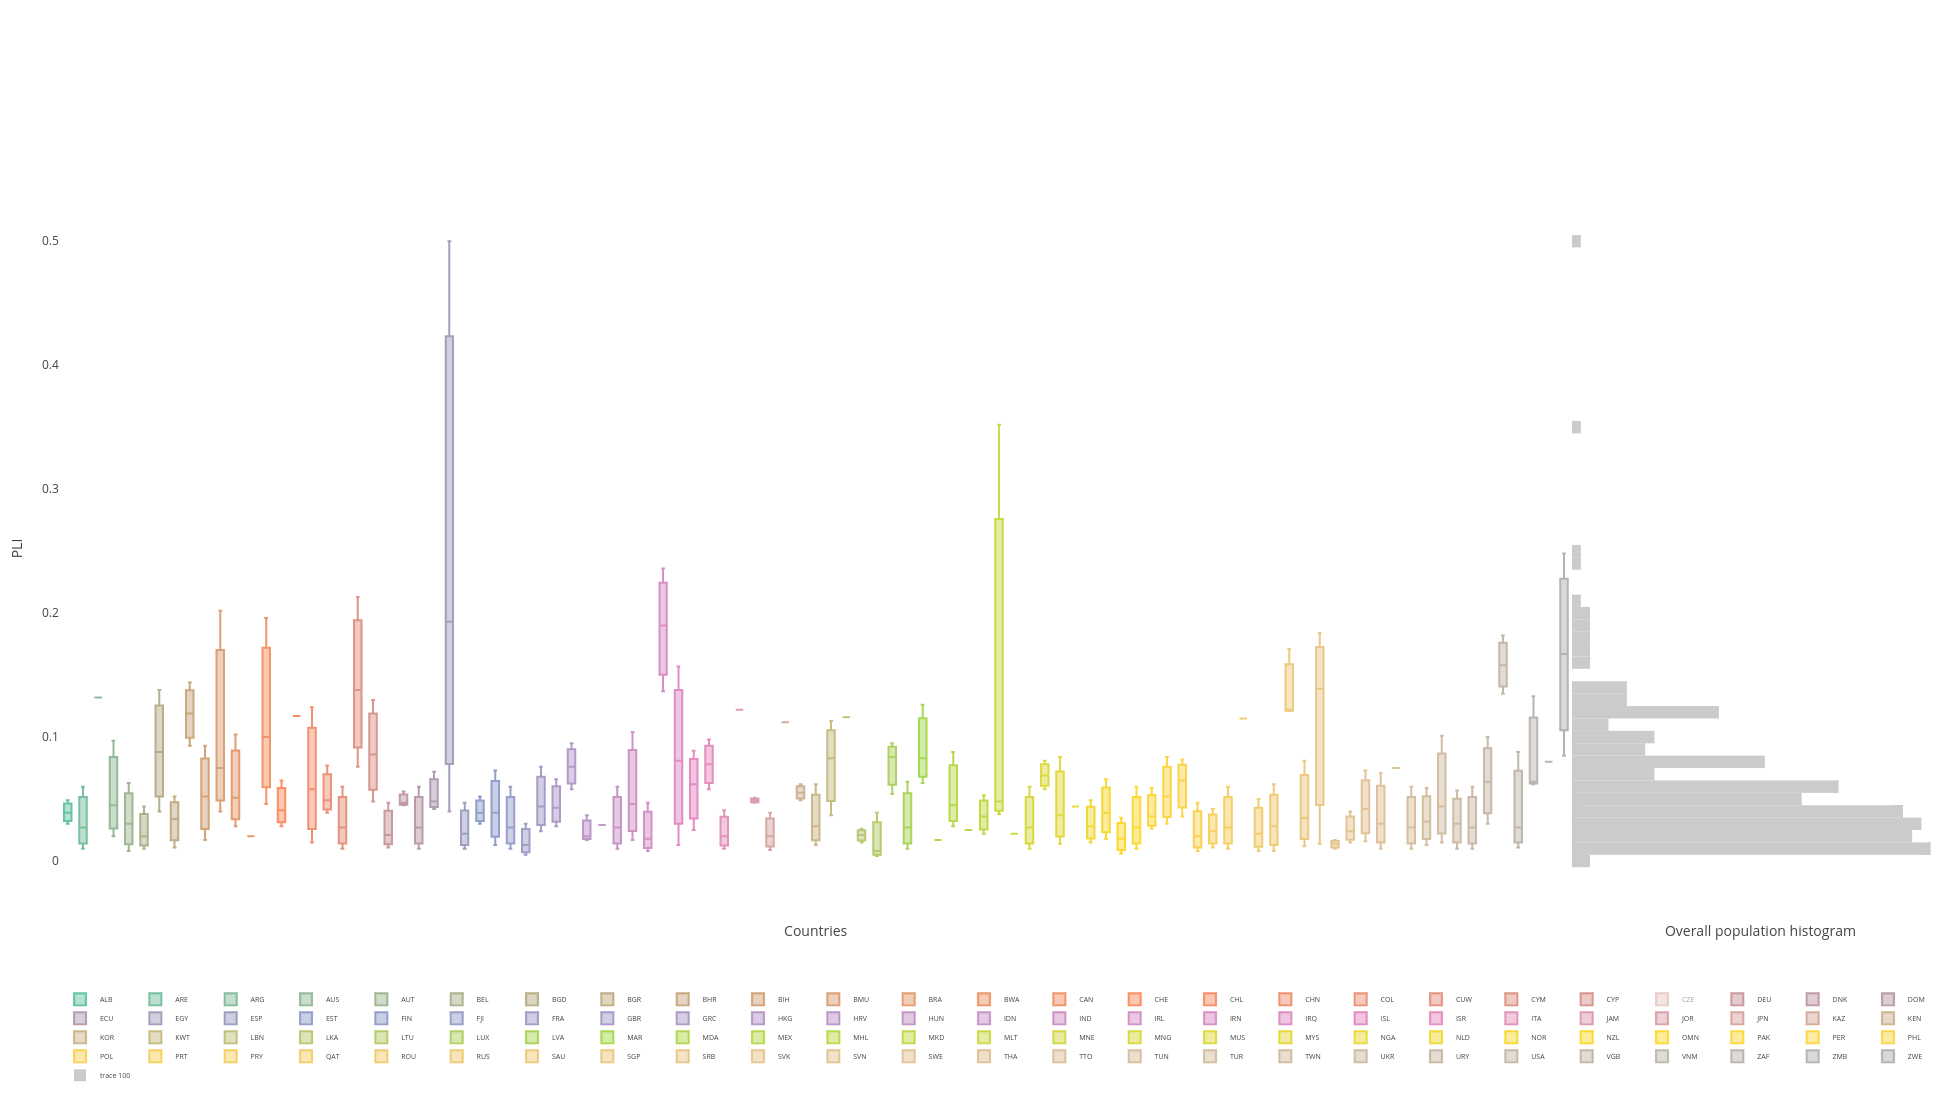
\includegraphics[width=\textwidth]{Images/plidist.png}
\caption{Interquartile range of distribution PLI sorted by country}
\end{figure}

In this figure, we can see how the PLI interquartile range changes from country to country in such case the PLI we choose was an ROS applied on independent companies whose activities are based on distribution (from wholesale to retail). Such difference can play a major role in deciding the optimal profitability level of the allocated entities. The PLI, acronym of Profit Level Indicator is the a financial indicator (most of the time a ratio) that tracks the profitability of a certain function performed by the entity under scope of analysis.

\subsection{Objectives}
The data reported above will be used to set up the GP model and constitutes part of the objectives and constraints that will be presented below. In order to model the overall allocation we need to take into consideration the following:
\begin{itemize}
    \item The overall cost of production should be minimized;
    \item The tax liability should be minimized;
    \item The profit should be divided among the entities based on the contribution that such entity give to the overall process of value creation;
    \item The functional characterization of each entity must fall within a range achieved by comparable non controlled entities.
\end{itemize}

\subsubsection{Cost minimization}
This is a very basic objective in which we try to minimize the cost embodied in each national entity. The cost function for each entity is primarily given by three variables, namely employees (which constitute the major variable cost of an enterprise) then we have the specific cost of running the assets (machinery, offices etc...) and then we have the cost of capital (meaning the remuneration expected share holders and financiers). All these variables contribute to the determination of costs. The approximation function derived will look as follows:

\[
C(E,A,K)=ce_k\cdot E+ca_k\cdot A+ck_k\cdot K \quad \forall k \in \left\{1...N\right\}
\]

Where (1)$ce_n$ corresponds to the National Income per Capita, this index was chosen because of its availability through the nations at scope and because it's a good proxy for the cost of labour in each State; (2)$ca_n$ corresponds to the cost of running the assets and is derived as illustrate before by subtracting the wage cost to the operational expenses and then adjusting for the purchasing power; (3)$ck_n$ corresponds to the cost of capital (in our case debt) calculated using data from comparable companies.
Even if this three variables do not represent the full cost structure of each enterprise (cost of good sold was not mentioned) is helpful for the decision maker to take into account this three driver of cost since this information constitutes the main driver to address value adding activities in the overall value chain.

\subsubsection{Tax base minimization}
This objective is the crucial point of this work since an optimal tax strategy can be considered good for profit maximization. However, should be mentioned that this doesn't constitute any avoidance of taxes but a strategy to be competitive in the market. Such allocation result as the consolidate minimization of all the national tax base, which is given by subtracting from the revenues allocated to a particular State ($y_k \cdot R$) the cost allocated to the same State (here expressed as $x_k \cdot C(E, A,K)$. This residual forms the EBIT (namely Earnings Before Interest and Taxes), by multiplying this the EBIT by the national corporate tax we get the Tax Base. The tax base function will look as follows:

\[
T(R,E,A,K)= [R-(ce_k\cdot E+ca_k\cdot A+ck_k\cdot K)]\cdot tx_k \quad \forall k \in \left\{1...N\right\}
\]

\subsubsection{Functional allocation}
This objective derives from the TNMM technique used in accessing the transfer pricing goodness. The method is based on the examination of the net profit relative to an appropriate base (e.g. costs, sales, assets) that a local entity realizes from a controlled transaction (or in our case to the entity itself). Basically, we introduced this objective as a quality control that the overall process of maximization of profits as some confirmation also in the real market, made by independent actors. This is in certain sense a bond that helps the model in giving a solution viable also in an anti avoidance perspective.

In order to do so we first need to identify which Profit Level Indicator to choose; this is an important choice that has to be made taking into account the functional characterization of such entity, that is, if an entity focuses on distribution the best PLI to test such entity is given by the ROS of its functional characteristics, that's because the sales are supposed to be the main element of a distributor (and not cost or assets). The main PLI used by practitioner are: Return on Sales, Full Cost Mark-up, Return on Asset, Return on Investment.

After we matched each functional characteristic with its relative PLI we need to find the data of comparable independent entities, in order to asses the profitability range that our entity has to obtain to be in an arm's length position.

The objective function returning such objective would be as follows:

\[
\begin{cases}
   \frac{R - C(E,A,K)}{R} & \text{if } q=1
   \\
   \frac{R - C(E,A,K)}{C(E,A,K)} & \text{if } q=2
   \\
   \frac{R - C(E,A,K)}{A} & \text{if } q=3
   \\
   \frac{R - C(E,A,K)}{E} & \text{if } q=4
\end{cases}
\]
The basic idea behind this objective is that for a moment we're forgetting about the group objective (the first and the second) that try to minimize the consolidated cost and tax base. In this case we're focusing on the profitability of each entity.

\subsection{Profit split}
This objective is represented by the goals (4)(5)(6) and the methodology used to determine this type of split derives from the profit split method used in transfer pricing analysis. In particular the transfer pricing profit split aims at: determining the division of profits that independent enterprises would have expected to realize from engaging in the transaction \cite{oecd_oecd_????}. In our case we'll use this method and particularly the contribution analysis to define the effort of each functional category in the value chain. Secondly we'll use this value driver to partition the profits in order to have, at the en, a structure that takes into account the internal value chain of the products and not just the information gained by independent comparable companies.

\subsection{Constraints}
Constraints represent the boundaries where the system will result unfeasible. Such constraints are expressed by the equation from (7) to (15); where the first two represent the boundaries on the PLI distribution namely the lower quartile and the upper quartile, outside this range the profitability may not be considered to be arm's length. The constraints (10)(11)(12)(13) represent the frontier of the possible allocable resources given by the company under the scope. The constraints (13),(14) and (15) sets the positiveness of the deviation variables in order to avoid incorrectness of the overall GP model. 

\subsection{Goal Programming Model}

This model aims to find the best allocation of costs and budgeted revenue in order to maximize profits minimizing costs and tax base, at the same time the model provides the best multinational functional allocation strategy to achieve such goal using both internal and external data from independent companies. 
The objectives are divided into two categories; the first one is given by three objectives namely cost minimization, tax base minimization, PLI coherence; the second focuses more on the control and limitations that the decision maker wants to implement in the model due to the specific characteristics of its business.

The overall model algebraically looks as follows:

\[ \min_{p,n} \quad \sum_{i=1}^{Q} (\prescript{}{q}{p}_i \cdot w_i) + w_3 \cdot \sum_{i=1}^{O} (\prescript{}{o}{n}_i) + w_4 \cdot \sum_{i=1}^{N} ( \prescript{}{n}{n}_i + \prescript{}{n}{p}_i )\]


\begin{numcases}{Subject \quad to}
   \sum_{q=1}^{N} C_q(E,A,K) - \prescript{}{q}{p}_1 = 0
   \\
   \sum_{q=1}^{N} T_q(R,E,A,K) - \prescript{}{q}{p}_2 = 0 
   \\
   P_k(R,E,A,K)+\prescript{}{n}{n}_k-\prescript{}{n}{p}_k =V_k  \qquad \forall k \in \left\{1...N\right\}
   \\
    \sum_{q=1}^{D} (R_q-C_q(E,A,K))+\prescript{}{o}{n}_1 = c_1\cdot \sum_{q=1}^{N} (R_q-C_q(E,A,K))  
   \\
    \sum_{q=1}^{P} (R_q-C_q(E,A,K))+\prescript{}{o}{n}_2 = c_2\cdot \sum_{q=1}^{N} (R_q-C_q(E,A,K)) 
   \\
    \sum_{q=1}^{M} (R_q-C_q(E,A,K))+\prescript{}{o}{n}_3 = c_3\cdot \sum_{i=q}^{N} (R_q-C_q(E,A,K)) 
   \\
   P_k(R,E,A,K) \geq L_k  \qquad \forall k \in \left\{1...N\right\}
   \\
   P_k(R,E,A,K) \leq U_k \qquad \forall k \in \left\{1...N\right\}
   \\
   \sum_{q=1}^{N} R_q = R^*
   \\
   \sum_{q=1}^{N} E_q = E^*
   \\
   \sum_{q=1}^{N} A_q = A^*
   \\
   \sum_{q=1}^{N} K_q = K^*
   \\
   \prescript{}{q}{p}_i,\prescript{}{q}{n}_i \geq 0 \qquad i=1,...,Q
   \\
   \prescript{}{n}{p}_i,\prescript{}{n}{n}_i \geq 0 \qquad i=1,...,N
   \\
   \prescript{}{o}{p}_i,\prescript{}{o}{n}_i \geq 0 \qquad i=1,...,O
 \end{numcases}


As you can see the (1)(2)(3) belong to the first category, where instead (4)(5)(6) belong to the second, the latter in fact depend on the strategy of the decision maker and it's not given by any environmental variable.

\section{Mathematical simulation: a case study}
The simulation of the above-mentioned model was made using LINGO17. Even if the mathematical package was able to handle the total amount of data given by the model the simulation was done using a portion of this data, avoiding countries in which the company doesn't operate at all. Other limitations were implemented in order to avoid any possible nonlinearity, resulting in an increase of the computational time to obtain a solution, this was possible by avoiding inserting the equation (3), when instead the correlated constraints, namely (7) and (8) were linearized. Other limitations to the model are exposed below:
\begin{itemize}
    \item The PLI chosen to set the functional range were only 2, ROS and FCMU;
    \item The cost of asset and equity was set to 0, meaning that the only cost driver was employees;
    \item The functional characterization was reduced to 3, namely distributor, producer and principal (which acts as an active holding);
    \item The number of employees was assumed to be continuous, meaning that part-time work and non full year worker can be used by the firm.
\end{itemize}

Concerning the data, the financial were taken from a company operating mostly in Europe and western countries in general, plus this company tend to produce and store most of its products in Asian countries and tend to have less inventory in its western distribution sites. The company under scope was under performing at the time of this simulation its P/L statement registered a loss of roughly  6.960.502 USD. The revenues registered for the year under the scope were about 88.900.344,00 USD and the employees hired were 2.722,00.
The weights were chosen in order to value firstly the tax minimization, then the contribution of each entity on the profit made by the company (profit split) and the cost minimization.

\subsection{Conclusions}
The results produced by the mathematical package are illustrated in the following table:

\begin{center}
 \begin{tabular}{||c c c c||} 
 \hline
 State & Function & Revenues allocation & Employees allocation \\ [0.5ex] 
 \hline\hline
 Cyprus & Distributor & 7.986.031 & 269,2824 \\ 
 \hline
 Denmark & Manufacturer & 5.464.000 & 57,5619 \\
 \hline
 Latvia & Principal & 64.144.930 & 2.295,3010 \\
 \hline
 Portugal & Principal & 11.305.390 & 99,8544 \\
 \hline
\end{tabular}
\end{center}

The financial data of the company shown an average consolidated tax burden of 21\% where instead using the model we achieved a rate of 17\% the only periods where such a ratio where lesser than the one achieved by the model where the one in which the company started to register losses (that caused a decrease in the tax burden). This model, fixing the PLI at a positive level doesn't allow any combination to result in an EBIT of 0 consequently the only achievable 0 rate may be in case of a tax haven.

The deviation variables we used registered the following discrepancies:

\begin{center}
\begin{tabular}{|| L  L L ||}
\hline
\text{Variable} & \text{Amount} & \text{Description} \\
\hline
\prescript{}{q}{p}_1 & 46.870.020,00 & \text{Consolidated cost of employees} \\
\hline
\prescript{}{q}{p}_2 & 7.159.194,00 & \text{Consolidated tax liability} \\
\hline
\prescript{}{o}{n}_1 & 0,00 & \text{Distributor profit allocation} \\
\hline
\prescript{}{o}{n}_2 & 0,00 & \text{Manufacturer profit allocation} \\
\hline
\prescript{}{o}{n}_3 & 0,00 & \text{Principal profit allocation} \\
\hline
\end{tabular}
\end{center}

The model is far from being used as the only tool that decision makers can use to solve problems of business restructuring, however, the result shows that multi criteria analysis and especially goal programming may constitutes one of the best tools that can be used to measure such decision.


\newpage
\emergencystretch=1em
\sloppy
\printbibliography
\end{document}